\documentclass{beamer}
\usetheme{Boadilla}
% 
\title{Modelling of crowd systems}
% \subtitle{Analysis of different models}
% \subtitle{Defining the problem}
\subtitle{Project Proposal review}
\author{D Purnendra Reddy}

\begin{document}
	\titlepage
{Prof. Pallab Sinha Mahapatra}

\begin{frame}	\frametitle{The problem - Objectives}
	In a dense crowding scenario, evacuation efficiency places a significant role in preventing disasters.
	    \begin{figure}
    \centering
        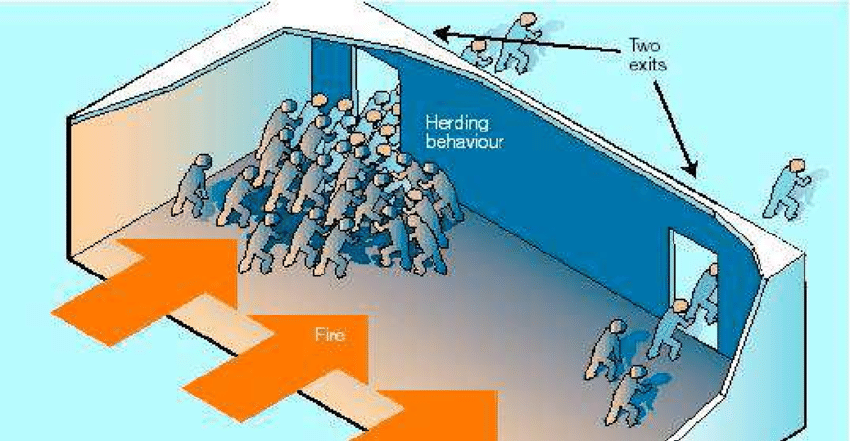
\includegraphics[width=0.5\textwidth]{crowd_panic.png}
    \end{figure}

	\begin{itemize}
	\item{\textbf{Option-1:}} Make exits wider and design better evacuation routes.
	\item{\textbf{Option-2:}} Obstacle phenomenon-	Impact of placing an obstacle at the upstream of exit. (\tiny preventing dense localisation of the crowd) 
	\begin{itemize} \scriptsize
		\item Relative dimensions to the exit
		\item Proximity to the exit 
		\item Lateral shift in Obstacle placement from the central line of the exit
		\item Shape of the obstacle
	\end{itemize}
	\end{itemize}
	Problem: Unsupervised crowd evacuation

	% \textbf{Objectives}
	% \begin{enumerate}
		% \item Time optimisation: Prevention of clogging near exits speeding up the evacuation process.
		% \item Minimal cost of obstacle placement - simplicity of shapes 
		% \item Ensure crowd pressures do not exceed dangerous limits close to the exit
		% \item Identify and define parameters that define evacuation efficiency.
	% \end{enumerate}
\end{frame}

\begin{frame}	\frametitle{Literature review}
	% Discussion
	% \begin{itemize}
		% \item 
	% \end{itemize}
	Critical Issues observed
	\begin{itemize}
		\item \textbf{Uncertainty of correlation and obstacle performance.}
		\begin{itemize}\scriptsize
			\item \textbf{Positive}: Prevents friction between crowd agents near the exit to avoid stop and go turbulent waves.
			\footnote[frame]{\tiny Zhao, Y., Li, M., Lu, X., Tian, L., Yu, Z., Huang, K., Wang, Y., Li, T., 2017. Optimal layout design of obstacles for panic evacuation using differential evolution. Phys. A: Stat.Mech. Appl. 465, 175–194.}
			\item \textbf{Negative}: Reduces effective exit area decreasing crowd outflow.
		\end{itemize}
		\item \textbf{Obstacle Performance.}
		\begin{itemize}\scriptsize
			\item Understanding the underlying mechanisms of obstacle effect that influence the outflow of crowd at bottlenecks.			\footnote[frame]{\tiny Zhongjun Ding et al J. Stat. Mech. (2020) 023404}
			\item Used cellular automaton model(Floor field) to arrive at the parameters that doesn't simulate real conditions as each person is restricted to a node and 8 possible directions.
			\footnote[frame]{\tiny Lei Wang et al 2016 Chinese Phys. B 25 118901}
		\end{itemize}
	\end{itemize}
\begin{columns}
\begin{column}{0.3\textwidth}
    \begin{figure}
    \centering
        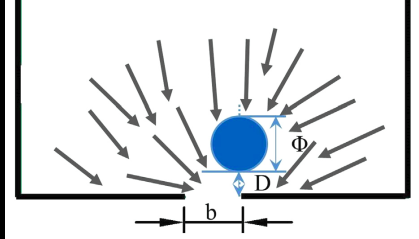
\includegraphics[width=1\textwidth]{obstacle_performanc.png}
    \end{figure}
\end{column}
\begin{column}{0.2\textwidth}
   \begin{figure}
    \centering
        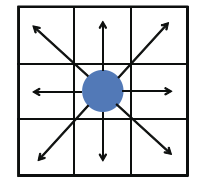
\includegraphics[width=1\textwidth]{nodal_analysis.png}
    \end{figure}
\end{column}
\end{columns}



		% \begin{itemize}
			% \item \textbf{Outdoor scenario:} Scope to study pedestrian streams in outdoor intersections or public squares by controlling the roundabout traffic in intersecting pedestrian streams. \footnote[frame]{\tiny Shiwakoti, N., 2010. Crowd Dynamics Under Emergency Conditions: Using Non-human Organisms in the Development of a Pedestrian Crowd Model. Ph.D. Thesis. Monash University.}
		% \end{itemize}
\end{frame}


\begin{frame}    \frametitle{Methodology- Multi Agent System}
\begin{columns}
\begin{column}{0.4\textwidth}
    \begin{figure}
    \centering
        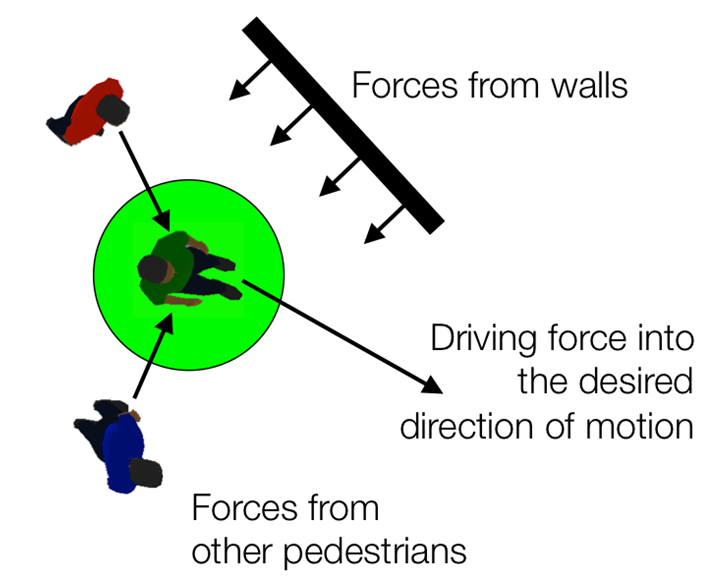
\includegraphics[width=1\textwidth]{social_force.png}
        \caption{Social Force model\footnote[frame]{\tiny Laufer, Julian(2022). Passenger and Pedestrian Modelling at Transport Facilities. }}
    \end{figure}
\end{column}
\begin{column}{0.6\textwidth}
	\begin{itemize}
	\item Approach to Model:
	\begin{itemize}\scriptsize
		\item Evacuating a crowd from a room through a single exit.
		\item Motion of a crowd agent determined through the superposition of forces from other agents and walls.
		\item A driving force guides the agent to move towards their destination. 
		\item Arrive at parameters that determine crowd pressure and turbulence.
	\end{itemize}
	\item Approach to Obstacles:
	\begin{itemize}\scriptsize
		\item Standard obstacles like cylindrical columns are discretised as wall elements to estimate their force field.
		\item Model is tested on obstacles under different test conditions.
	\end{itemize}
	\end{itemize}
\end{column}
\end{columns}

\end{frame}

\begin{frame}
\frametitle{Using Social Force model}
  \[m_i\frac{d v_i}{dt} = F_i^{desired}+F_{iw}^{obstacle}+F_{ij}^{pedestrian}\]
      \[F_i^{desired}=m_i \frac{[v_{i_{max}}^o(t)-v_i(t)]}{\tau}\]

    \small \[F_{ij}^{pedestrian}=we^{\frac{r_{ij}-d_{ij}}{w}}(\lambda+(1-\lambda)(\frac{1+cos\omega_i}{2}) \bar n_{ij} + \mu g(r_{ij}-d_{ij}) \Delta \bar v_{ij}(t)+w*(r_{ij}-d_{ij}) \bar n_{ij} \]
        
      \[F_{io}^{obstacle}=w.e^{\frac{r_{i}-d_{io}}{w}} \bar n_{io} + \mu g(r_{i}-d_{io}) \Delta \bar v_{io}(t)  + w*(r_{i}-d_{io}) \bar n_{io} \]

\end{frame}

\begin{frame}    \frametitle{Summary of Work done}
\begin{columns}
\begin{column}{0.4\textwidth}
    \begin{figure}
    \centering
        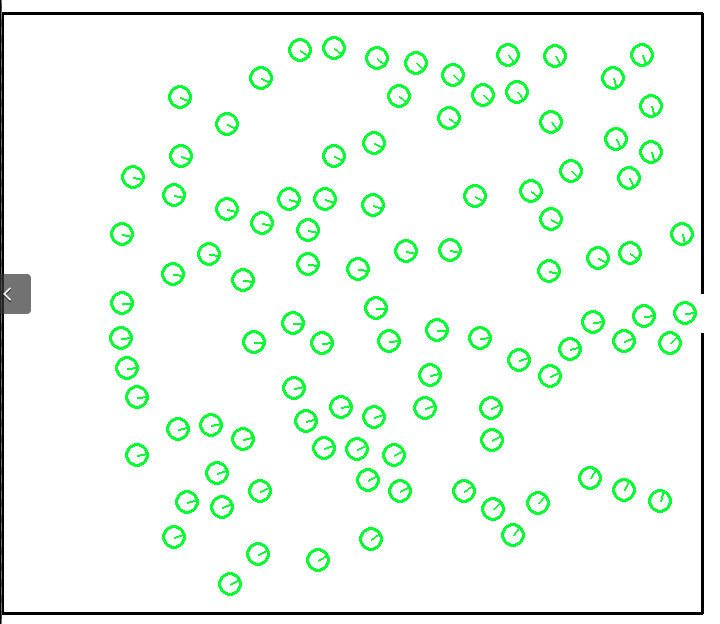
\includegraphics[width=1\textwidth]{work_summary.png}
        \caption{Simulation}
    \end{figure}
\end{column}
\begin{column}{0.6\textwidth}
	\begin{itemize}
		\item Completed Literature review.
		\item Modelled a crowd evacuation scenario without obstacles using python3.
		\item Working on validation of Helbing's social force model.
	\end{itemize}
\end{column}
\end{columns}

\end{frame}

\begin{frame}    \frametitle{Future Timeline}
\begin{itemize}
	\item \textbf{JUN-AUG} Conceptual Understanding,Literature review \& Code development 
	\item \textbf{SEP-DEC}
	\begin{itemize}
		\item Code development \& Simulation
		\item Validation of model
		\item Identification of crowd dense areas near the exit
		\item Placement of obstacles and Data collection  
		% \item Parameter optimisation
	\end{itemize}
	\item \textbf{JAN-MAR} 
	\begin{itemize}
		\item Identification of Parameters influencing evacuation behaviour, it's optimisation and correlation  
	\end{itemize}
	\item \textbf{APR} Report
\end{itemize}
\end{frame}
\end{document} 	

